
\documentclass[a4paper,12pt]{article}
\usepackage[ngerman]{babel}
% \usepackage[ngerman]{babel}
\usepackage[utf8]{inputenc}
\usepackage[T1]{fontenc}
\usepackage{lmodern}
\usepackage{titling}
\usepackage{geometry}
\geometry{left=3cm, right=3cm, top=2cm, bottom=3cm}
\usepackage{setspace}
\onehalfspacing

\usepackage{ifthen}

\usepackage{graphicx}
% \usepackage{pstricks}
% \usepackage{relsize}
% \usepackage[decimalsymbol=comma,exponent-product = \cdot, per=frac]{siunitx}
% \sisetup{range-phrase=\,bis\,}

\usepackage{xargs}
\usepackage{calc}
\usepackage{amsmath}
\usepackage{amsfonts}
\usepackage{mathtools}
\usepackage{amssymb}

\usepackage{cancel}
\usepackage{trfsigns}
\usepackage{array}
\usepackage{enumerate}
\usepackage{enumitem}

\usepackage{caption}
\usepackage{subcaption}

\usepackage{multicol}

\usepackage{pdflscape}
\usepackage[table]{xcolor}

\usepackage{float}

%%%%%%%%%%%%%%%%%%%%%%%%%%%%%%%%%%%%%%%%%%%%%%%%%%%%%%%%%%%%%%%%%%%%%%%%%%%%%%%%
\newboolean{WITHPSTRICKS}
\setboolean{WITHPSTRICKS}{false}


\newcommand{\PROFESSOR}{Prof.\ Dr.\ Thomas Carraro}
\newcommand{\ASSISTANT}{\setlength{\tabcolsep}{0pt}\begin{tabular}{l} Dr. Ulrike Kochan-Eilers\end{tabular}}

\newcommand{\Jahr}{2025}
% \newcommand{\Trimester}{HT}
\newcommand{\Trimester}{WT}
\newcommand{\Kurs}{Mathematik II/B (WI/ET)}
\newcommand{\TYPE}{Aufgabenblatt}
\newcommand{\BLATT}{8}
\newcommand{\TOPIC}{partielle Ableitungen, Richtungsableitung, Tangentialebene, station\"are Punkte}

%%%%%%%%%%%%%%%%%%%%%%%%%%%%%%%%%%%%%%%%%%%%%%%%%%%%%%%%%%%%%%%%%%%%%%%%%%%%%%%%
\newboolean{mitLoes}
\setboolean{mitLoes}{false}
\setboolean{mitLoes}{true}

%%%%%%%%%%%%%%%%%%%%%%%%%%%%%%%%%%%%%%%%%%%%%%%%%%%%%%%%%%%%%%%%%%%%%%%%%%%%%%%%


%\setboolean{WITHPSTRICKS}{false}
\setboolean{WITHPSTRICKS}{true}


\usepackage{tikz}
\usetikzlibrary{arrows,automata,backgrounds,calendar,decorations.pathmorphing,fadings,shadings,calc,intersections}
\usetikzlibrary{decorations.pathreplacing}
\usetikzlibrary{decorations.shapes}
\usetikzlibrary{decorations.footprints}
\usetikzlibrary{decorations.text}
\usetikzlibrary{positioning}
\usetikzlibrary{through}

\ifthenelse{\boolean{WITHPSTRICKS}}{%
\usepackage{auto-pst-pdf}
\usepackage{pstricks,pst-plot,pst-text}
}{}

\usepackage{pgfplots}

%%%%%%%%%%%%%%%%%%%%%%%%%%%%%%%%%%%%%%%%%%%%%%%%%%%%%%%%%%%%%%%%%%%%%%%%%%%%%%%%
\usepackage{mbdefAufgaben}

%%%%%%%%%%%%%%%%%%%%%%%%%%%%%%%%%%%%%%%%%%%%%%%%%%%%%%%%%%%%%%%%%%%%%%%%%%%%%%%%
\newboolean{mitErg}
\setboolean{mitErg}{false}

%%%%%%%%%%%%%%%%%%%%%%%%%%%%%%%%%%%%%%%%%%%%%%%%%%%%%%%%%%%%%%%%%%%%%%%%%%%%%%%%
\newcounter{Aufg}
\setcounter{Aufg}{0}
\newcounter{Blatt}
\setcounter{Blatt}{\BLATT}

%%%%%%%%%%%%%%%%%%%%%%%%%%%%%%%%%%%%%%%%%%%%%%%%%%%%%%%%%%%%%%%%%%%%%%%%%%%%%%%%
\usepackage{KopfEnglish}

% Seitenraender
\textwidth = 285mm
\textheight = 180mm
\leftmargin 5mm
\oddsidemargin = -20mm
\evensidemargin = -20mm
\topmargin = -25mm
\parindent 0cm
\columnsep 2cm

% % % Aufgabenstellung
% % % Schwierungkeitsgrad mit "e" , "f" oder "v" angeben
% % % "e" Einführung   
% % % "f" Festigung
% % % "v" Vertiefung  

\newcommand{\Aufgabe}[3][]{
\stepcounter{Aufg}
\subsubsection*{Aufgabe 
\arabic{Blatt}.\arabic{Aufg}\ifthenelse{\equal{#1}{e}}{}{\ifthenelse{\equal{#1}{f}}{
$\!\!{}^\star$}{\ifthenelse{\equal{#1}{v}}{$^{\star\star}$}{}}}{: #2}}
{#3}
}
% % % Ergebnisse jeweils am Ende des Aufgabenblattes Anzeigen
\newcommand{\Ergebnisse}{}
\makeatletter
\newcommand{\Ergebnis}[1]{
	\g@addto@macro{\Ergebnisse}{#1}
}
\makeatother
\makeatletter
\newcommand{\ErgebnisC}[2]{
\@ifundefined{c@#1}
{\newcounter{#1}}
{}
\setcounter{#1}{\theAufg}

\ifthenelse{\boolean{mitErg}}{	\g@addto@macro{\Ergebnisse}{\subsubsection*{Ergebnisse zu Aufgabe \arabic{Blatt}.\arabic{#1}:}
}%
	\g@addto@macro{\Ergebnisse}{#2}}{}
}
\makeatother


% % % Lösungen
\newcommand{\Loesung}[1]{
	\ifthenelse{\boolean{mitLoes}}
	{\subsubsection*{Lösung \arabic{Blatt}.\arabic{Aufg}:}
		#1}
	{}
}
% % % % % % % % % % % % % % % % % % % % % % % % % % % % % % % % % % % % % % % % % % % % % % % % % % % % % %
% % % % % % % % % % % % % % % % % % % % % % % % % % % % % % % % % % % % % % % % % % % % % % % % % % % % % %
% % % % % % % % % % % % % % % % % % % % % % % % % % % % % % % % % % % % % % % % % % % % % % % % % % % % % %
\begin{document}
\begin{twocolumn}
% % % % % % % % % % % % % % % % % % % % % % % % % % %

%%%%%%%%%%%%%%%%%%%%%%%%%%%%%%%%%%%%%%%%%%%%%%%%%%%%%%%%%%%%%%%%%%%%%%%%%%%%%%%%
% Set the TITLE of the sheet here:
%\uebheader{\Kurs}{\arabic{Blatt}}{\Trimester\,\Jahr}{\TOPIC}
%\uebheader{\Kurs}{\arabic{Blatt}}{\Trimester\,\Jahr}{\TOPIC}
\uebheader{\Kurs}{\arabic{Blatt}}{\Trimester\,\Jahr}{\TOPIC}
\ruleBig

\setboolean{mitErg}{false}
\setboolean{mitErg}{true}


%%%%%%%%%%%%%%%%%%%%%%%%%%%%%%%%%%%%%%%%%%%%%%%%%%%%%%%%%%%%%%%%%%%%%%%%%%%%%%%%
% Set the INTRODUCTION section of the sheet here:
% \input{introduction.tex}

\textbf{Einführende Bemerkungen}

\begin{itemize}
\item Vermeiden Sie die Verwendung von Taschenrechnern oder Online-Ressourcen.
% \item Die mit einem Stern *) markierten (Teil-)Aufgaben entfallen in diesem Trimester. Stattdessen werden einzelne Online-Aufgaben im ILIAS-Kurs kenntlich gemacht, zu denen Sie dort Ihre L\"osungswege zur Korrektur hochladen k\"onnen. 
% \item Die mit zwei Sternen  **) markierten (Teil-)Aufgaben richten sich an Studierende, die die \"ubrigen Aufgaben bereits gel\"ost haben und die Inhalte weiter vertiefen m\"ochten. 
\end{itemize}

\ruleBig

%Mathe VIII Blatt 
%
%9
\Aufgabe[]{}
{
Bestimmen und klassifizieren Sie alle station\"aren Punkte der Funktion 
$$g(x,y)=3x^2-2xy-\dfrac{y^3}6. $$
}

\Loesung{
Die ersten beiden Ableitungen von $g$ sind gegeben durch 
$$\nabla g(x,y)=\begin{pmatrix}6x-2y\\-2x-y^2/2\end{pmatrix}\text{ und }\vec H_g(x,y)= \begin{pmatrix} 6 & -2\\ -2 & -y\end{pmatrix}.$$
An den station\"aren Punkten gilt 
\begin{align*}
&&\vec 0=&\nabla g(x,y)=\begin{pmatrix}6x-2y\\-2x-y^2/2\end{pmatrix}\\
\Leftrightarrow&& y=& 3x,\, 9x^2+4x=0\\
\Leftrightarrow&& (x,y)=& (0,0)\text{ oder } (x,y)=\left( -\frac 49,-\frac43\right)
\end{align*}
Um die Punkte zu charakterisieren wird dort die Hessematrix berechnet. Im ersten Punkt ist 
$$\vec H_g(0,0)=\begin{pmatrix} 6 & -2\\ -2 & 0\end{pmatrix}.$$
Diese Matrix ist indefinit, denn die Eigenwerte sind:
$$
\lambda_1 = 3 + \sqrt{13} > 0 \quad \text{ und } \quad \lambda_2 = 3 - \sqrt{13} < 0 .
$$
Alternativ kann man die Indefinitheit zeigen durch
$$(1,0) \vec H_g(0,0)\begin{pmatrix}1\\0\end{pmatrix} = 6>0$$ 
und andererseits
$$(1,2) \vec H_g(0,0)\begin{pmatrix}1\\2\end{pmatrix}=-2<0.$$
Im Ursprung liegt also ein Sattelpunkt. \\
Im zweiten Punkt ist 
$$\vec H_g(-4/9,-4/3)=\begin{pmatrix} 6 & -2\\ -2 & \frac{4}{3}\end{pmatrix}.$$
Diese Matrix ist diagonaldominant mit positiven Diagonalelementen, also positiv definit, somit liegt im Punkt $(-4/9,-4/3)$  ein Minimum. 
Die positive Definitheit kann auch \"uber die Eigenwerte gezeigt werden. Die Eigenwerte sind:
$$
\lambda_1 = \frac13(11 + \sqrt{85}) > 0 \quad \text{ und } \quad \lambda_2 = \frac13 ( 11 - \sqrt{85}) > 0 .
$$
}


\ErgebnisC{analysDiffNdim14a}{
$\vec x_1=(0,0)^\top,\, \vec x_2=(-4/9,-4/3)^\top$
}

\ifthenelse{\boolean{mitLoes}}{\ruleBig \cleardoublepage}{}

%17
\Aufgabe[e]{Stationäre Punkte}{
Gegeben sei die Funktion $$f(x,y) = x^3+x^2y-y^2-4y.$$ Finde alle stationären Punkte und bestimme, ob sie lokale Minima, Maxima oder Sattelpunkte sind.
}
\Loesung{
Die stationären Punkte sind die Lösungen des folgenden Gleichungssystems%
\begin{eqnarray*}
\frac{\partial}{\partial x} f(x,y) = 0 \quad&\Rightarrow& \quad x(3x+2y)= 0 \\\
\frac{\partial}{\partial y} f(x,y) = 0 \quad&\Rightarrow& \quad x^2-2y-4= 0
\end{eqnarray*}
%
Die erste Gleichung ist für $x=0$ und für $3x+2y=0$ erfüllt, d.h. wenn $x=0$ oder wenn $y=-\frac32 x$. In beiden Fällen wird der $y$-Wert durch die zweite Gleichung im System bestimmt.
\begin{enumerate}
\item Fall $x=0$: Aus der zweiten Gleichung ergibt sich $0-2y-4=0$, d.h. \ $y=-2$. Der erste kritische Punkt ist $\vec P_1 = (0,-2)$.
\item Fall $y=-\frac32 x$. Setzt man dies in die zweite Gleichung ein, erhält man $x^2-2(-\frac32 x) - 4 =0$. Dies ergibt
$$
x^2+3x-4=0 \longrightarrow (x-1)(x+4)=0.
$$
Die Lösungen sind $x=1$ und $x=-4$. Die beiden weiteren kritischen Punkte sind dann: $\vec P_2=(1,-\frac32)$ und $\vec P_3=(-4, 6)$.
\end{enumerate}

Zusammengefasst lauten die drei kritischen Punkte
$$
\vec P_1 = (0,-2),\qquad \vec P_2 = (1,-\frac32), \qquad \vec P_3 = (-4,6).
$$

Die Hessische Matrix ist:
$$
H=
\begin{pmatrix}
f_{xx}(x,y) & f_{xy}(x,y) \\
f_{xy}(x,y) & f_{yy}(x,y) 
\end{pmatrix}
=
\begin{pmatrix}
6x+2y & 2x \\
2x & -2
\end{pmatrix}.
$$


Charakterisierung der stationären Punkte:
\begin{align*}
\boldsymbol{P}_1 &= \begin{pmatrix} 0 \\\ -2 \end{pmatrix}, \quad \begin{pmatrix} -4 & 0 \\\\ 0 & -2 \end{pmatrix}, \quad h_{11}<0, \det(H)=8>0 \rightarrow \mbox{Maximum}\\
\boldsymbol{P}_2 &= \begin{pmatrix} 1 \\\ -\frac32 \end{pmatrix}, \quad \begin{pmatrix} 3 & 2 \\\ 2 & -2 \end{pmatrix}, \quad h_{11}>0, \det(H)=-10<0 \rightarrow \mbox{Sattelpunkt}\\
\boldsymbol{P}_3 &= \begin{pmatrix} -4 \\\ 6 \end{pmatrix}, \quad \begin{pmatrix} -12 & -8 \\\ -8 & -2 \end{pmatrix}, \quad h_{11}<0, \det(H)=-40<0 \rightarrow \mbox{Sattelpunkt}
\end{align*}

}

\ifthenelse{\boolean{mitLoes}}{\ruleBig \cleardoublepage}{}

%20
\Aufgabe[e]{Station\"are Punkte} {
 Gegeben sei die Funktion
$$
f(x,y) =  ax^2 + 2xy + ay^2-ax-ay.
$$
Bestimmen Sie diejenigen $a\in \R$, f\"ur welche die Funktion 
$f$ relative Maxima, relative Minima und Sattelpunkte besitzt und geben Sie 
diese an. 
}

\Loesung{
In station\"aren Punkten  muss der Gradient der Funktion Null werden: 
\begin{align*}
&\vec 0= \nabla f(x,y)=\begin{pmatrix} 2ax+2y-a\\2x+2ay-a\end{pmatrix}\\
&\begin{array}{r|rr|r|l}
\mathrm{I}  & 2a     &    2 &     a& \mathrm{I'} = \mathrm{II}\\
\mathrm{II} & 2      &   2a &     a& \mathrm{II'} = \mathrm{I}\\\hline
\mathrm{I}' & 2      &   2a &     a&  \\
\mathrm{II'} & 2a     &    2 &     a&\mathrm{II''}= \mathrm{II'} -a\cdot \mathrm{I'}\\\hline
\mathrm{I'}& 2     &    2a &     a  & \mathrm{I''}= \mathrm{I'}: 2\\
\mathrm{II''}& 0     &    2-2a^2 &     a-a^2  & \mathrm{II'''} = \mathrm{II''} : (2-2a^2), \text{ f\"ur }a^2\neq 1\\\hline
\mathrm{I''}& 1     &    a & \frac a 2  & \\
\mathrm{II'''}& 0 &    1 & \frac{a(1-a)}{2(1-a^2)}\\
\end{array}
\end{align*}
Dann ist 
\begin{align*}
y &= \frac{a(1-a)}{2(1+a)(1-a)} = \frac{a}{2(1+a)}\\
x &= \frac{a}{2} - a \cdot \frac{a}{2(1+a)} = \frac{a(1+a-a)}{2(1+a)} = \frac{a}{2(1+a)}\,.
\end{align*}

F\"ur $a\neq \pm 1$ liegt der einzige kritische Punkt der Funktion also bei 
$$\vec x_0 = \begin{pmatrix} \frac{ a}{2(1+a)}\\ \frac{a}{2(1+a)}\end{pmatrix}. 
$$
F\"ur $a=+1$ hat das obige Gleichungssystem die L\"osung $(t,\frac 12 -t)$ ($t\in\R$). \\
F\"ur $a=-1$ hat das Gleichungssystem keine L\"osung und damit $f$ keinen station\"aren Punkt. \\
Zur Charakterisierung der station\"aren Punkte ben\"otigen wir die Hesse-Matrix: 
$$\vec H_f(x,y)=\begin{pmatrix} 2a& 2\\ 2 & 2a\end{pmatrix}.$$
Ihre Determinante ist \(\det (\vec H_f) = 4 (a^2-1)\).
Wir unterscheiden zun\"achst die drei F\"alle: 
\begin{iii}
\item $-1<a<1$: F\"ur die Determinante gilt \(\det(\vec H_f) < 0\). Da die Determinante aus dem Produkt der Eigenwerte berechnet wird, folgt daraus, dass die Eigenwerte verschiedene Vorzeichen haben. $\vec H_f$ ist indefinit und $\vec x_0$ ist ein
Sattelpunkt. 
\item $a<-1$: F\"ur die Determinante gilt \(\det(\vec H_f) > 0\). Daraus folgt, dass die Eigenwerte gleiches Vorzeichen haben. Da die Spur \(\operatorname{Sp}(\vec H_f) = 4 a\)  in diesem Fall negativ ist, sind die beiden Eigenwerte negativ. Also ist $\vec H_f$  negativ definit und die Funktion $f$ hat ein Maximum in $\vec x_0$. 
\item $1<a$: Sowohl die Determinante, als auch die Spur sind positiv. Deswegen sind beide Eigenwerte positiv und bei $\vec x_0$ ist ein Minimum. 
\end{iii}
F\"ur $a=1$ gilt \(\det(\vec H_f)=0\), also ist mindestens ein Eigenwert gleich Null. In diesem Fall gilt \[f(x,y) = x^2+2xy+y^2-x-y = (x+y)^2 - (x+y) = \left(x+y-\frac12\right)^2 - \frac14\,.\]
In allen station\"are Punkten $(t,\, \frac 12 -t)^\top$ ist der quadratische Term \((x+y-\frac12)^2\) gleich Null, aber in allen anderen Punkten ist er positiv. Deshalb liegt in diesen station\"aren Punkten ein Minimum vor. Diese Punkte
befinden sich auf einer Geraden, auf der $f$ konstant ist. \\
Insgesamt besitzt die Funktion $f$ also 
\begin{itemize}
\item f\"ur $a<-1$ ein Maximum in $\vec x_0=\frac a{2(1+a)}(1,1)^\top$. 
\item f\"ur $a=-1$ keinen station\"aren Punkt. 
\item f\"ur $-1<a<1$ einen Sattelpunkt in $\vec x_0=\frac a{2(1+a)}(1,1)^\top$. 
\item f\"ur $a=1$ die Minimalstellen $(t,\, \frac 12 - t)^\top$, $t\in\R$. 
\item f\"ur $1<a$ ein Minimum in $\vec x_0=\frac a{2(1+a)}(1,1)^\top$. 
\end{itemize}
}

\ErgebnisC{AufganalysExtrNdim004}
{
{
F\"ur $a\neq \pm 1$ ist der station\"are Punkt $\frac a{2(1+a)}(1,1)^\top$. F\"ur $a=1$ gibt es
mehrere station\"are Punkte. 
}
}


\ifthenelse{\boolean{mitLoes}}{\ruleBig \cleardoublepage}{}

% 92
\Aufgabe[e]{Wegableitungen} {
Gegeben sind die Funktionen
$$f(x,y)=\EH x \cdot \sin y\text{ und }\vec g(t)=(t^3,\, 1+t^2)^\top$$
aus denen sich die Funktion $h(t)=f(\vec g(t))$ ergibt. 
\begin{abc}
\item Berechnen Sie $h'(t)$ durch explizites Einsetzen und anschließendes (eindimensionales)
Ableiten nach $t$. 
\item Berechnen Sie $h'(t)$ mit Hilfe der Kettenregel. 
\end{abc}

}


\Loesung{
\begin{abc}
\item 
\begin{align*}
h'(t) =&\frac{\text{d} }{\text{d} t} \left( f(t^3,1+t^2)\right) \\
=& \frac{\text{d} }{\text{d} t}\left( \EH{t^3} \cdot \sin(1+t^2)\right)\\
=& 3t^2 \EH{t^3}\cdot \sin(1+t^2)+\EH{t^3} \cdot 2t \cos(1+t^2)\\
=& \left(3t\sin(1+t^2)+2\cos(1+t^2)\right) t \EH{t^3}
\end{align*}
\item 
\begin{align*}
h'(t)=& \bigl(\nabla f(\vec g(t))\bigr)^\top \vec g'(t) \\
&=\bigl(\EH {g_1(t)} \sin (g_2(t)),\, \EH {g_1(t)} \cos(g_2(t)) \bigr) \begin{pmatrix} 3t^2\\2t\end{pmatrix}\\
=& \EH{t^3}\sin(1+t^2)\cdot 3t^2 + \EH{t^3}\cos(1+t^2)\cdot 2t\\
=&(3t\sin(1+t^2)+2\cos(1+t^2))t\EH{t^3}
\end{align*}
\end{abc}
}

\ErgebnisC{AufganalysWegAblt001}
{
$h'(t)=t\EH{(t^3)}\bigl( 3t\sin(t+t^2)+2\cos(1+t^2)\bigr)$
}

\ifthenelse{\boolean{mitLoes}}{\ruleBig \cleardoublepage}{}

% 95
\Aufgabe[e]{Lokale Extrema in 2 Dim.}
{
Gegeben sei die Funktion $f\in {\text{Abb}}\,(\R^2,\R)$ mit
\[
f(x,y)= (x+y)^2-4\,(x+y-2)+y^3-3y .
\]
Bestimmen Sie alle station\"aren (kritischen) Punkte dieser Funktion und geben Sie
an, ob es sich dabei um lokale Minima, Maxima oder Sattelpunkte handelt, oder ob
der Charakter des station\"aren Punktes nicht durch die Hesse--Matrix entschieden 
werden kann.
}
\Loesung{
Die station\"aren Punkte erh\"alt man aus
\[
	\textbf{grad}\,f(x,y) = \begin{pmatrix}
	                        2\,(x+y)-4 \\
	                        2\,(x+y)-4 +3\,y^2-3
	                        \end{pmatrix} = \begin{pmatrix}  0 \\ 0 \end{pmatrix} 
\]
zu \ $P_1 = (3,-1)$ \ und \ $P_2 = (1,1)$. Die Hesse--Matrix der Funktion 
\ $f$ \ lautet:
\[
	\vec{H}_f(x,y) = \begin{pmatrix}
	                     2 & & 2 \\
	                     2 & & 2+6\,y
	                     \end{pmatrix}\,.
\]
Für den Punkt \ $P_1$ \ ergibt sich damit
\[
	\vec{H}_f(3,-1) = \begin{pmatrix} 2 & 2 \\ 2 & -4 \end{pmatrix} 
	\quad \Longrightarrow \lambda_1 \cdot \lambda_2 = \det(\vec H_f) = -12 < 0\ ,                   
\]
Damit haben die Eigenwerte verschiedene Vorzeichen und es handelt sich um einen Sattelpunkt. Entsprechend erh\"alt man für den 
Punkt \ $P_2$, dass 
	\[
	\vec{H}_f(1,1) = \begin{pmatrix} 2 & 2 \\ 2 & 8\end{pmatrix} 
	\quad \Longrightarrow \lambda_1 \cdot \lambda_2 = \det(\vec H_f) = 12 > 0,\, \operatorname{Sp}(\vec H_f) = 10 > 0\,.                   
\]
Damit sind beide Eigenwerte positiv und es handelt sich um ein Minimum.
}


\ErgebnisC{Aufgb-2011A-K-A4a}
{
Die station\"aren Punkte lauten  $P_1 = (3,-1)$ und $P_2 = (1,1)\,.$
}

\ifthenelse{\boolean{mitLoes}}{\ruleBig \cleardoublepage}{}

% 109
\Aufgabe[e]{Taylor--Entwicklung in 2 Dim.}{
Bestimmen Sie das Taylor-Polynom 2. Ordnung der Funktion 
$$
f(x,y) = \EH x\cos(\pi(x+2y))
$$
um den Entwicklungspunkt \ $\vec x_0 = (1,-1)^{\top}$ .
}

\Loesung{
Die partiellen Ableitungen lauten:
\begin{align*}
f(x,y) =& \EH x\cdot\cos\big(\pi(x+2y)\big) \\
&\,\Rightarrow\, f(1,-1) =-\EH{ } \\
\\
f_x(x,y) =& \EH x\cdot \Big[\cos\big(\pi(x+2y)\big) -\pi\sin\big(\pi(x+2y)\big) \Big] \\
&\,\Rightarrow\, f_x(1,-1) = -\EH{ } \\
\\
f_y(x,y) =& -2\pi\cdot\EH x\cdot \sin\big(\pi(x+2y)\big) \\
&\,\Rightarrow\, f_y(1,-1) = 0\\
\\
f_{xx}(x,y) =& \EH x \Big[(1-\pi^2)\cos\big(\pi(x+2y)\big) - 2\pi\sin\big(\pi(x+2y)\big)\Big] \\
&\,\Rightarrow\, f_{xx}(1,-1) =\EH{ }\,(\pi^2-1) \\
\\
f_{xy}(x,y) =& -2\pi\cdot \EH x \Big[\sin\big(\pi(x+2y)\big) + \pi\cos\big(\pi(x+2y)\big)\Big] \\
&\,\Rightarrow\, f_{xy}(1,-1) = 2\,\pi^2\,\EH{ } \\
\\
f_{yy}(x,y) =& -4\,\pi^2\cdot \EH x\cdot \cos\big(\pi(x+2y)\big) \\
&\,\Rightarrow\, f_{yy}(1,-1) = 4\,\pi^2\,\EH{ } \\
\end{align*}

Damit lautet das Taylorpolynom 2. Grades am Entwicklungspunkt \ $\vec x_0 =(1,-1)^{\top}$
\[
T_2(x,y) =  -\EH{ } - \EH{ }\,(x-1) + (\pi^2-1)\,\EH{ }\,\dfrac{(x-1)^2}{2} + 2\pi^2\,\EH{ }\,(x-1)(y+1)+ 4\pi^2\,\EH{ }\,\dfrac{(y+1)^2}{2} \ .
\]
}

% \ErgebnisC{dummy}
% {
% 
% }


\ifthenelse{\boolean{mitLoes}}{\ruleBig \cleardoublepage}{}

% 110
\Aufgabe[e]{Taylor--Entwicklung in 2 Dim.}{
Gegeben seien \ $f:\R^2 \to \R$  \ mit \ $f(x,y)=\EH{xy}+x+y$ \ und \ $\vec{a}=\dfrac{1}{5}\begin{pmatrix}{-4}\\{3}\end{pmatrix}$\,.

\begin{itemize}
\item[ a)] Bestimmen Sie das Taylorpolynom 2. Grades von \ $f$ \ für den Entwicklungspunkt \ $(0,0)$\,.
  
\item[ b)] Bestimmen Sie die Richtungsableitung \ $\partial$$_{\vec a}$$\,f$ \ von \ $f$ \ in Richtung \  $\vec{a}$ \ im Punkt \ $(0,0)$\,. 
\end{itemize}
}

\Loesung{
\textbf{a)} \ Mit den partiellen Ableitungen 
  \[
  \begin{array}{rclcl}
  f_x & = & y\,\EH{xy}+1 & \Rightarrow  & f_x(0,0)=1\ , \\
  f_y & = & x\,\EH{xy}+1 & \Rightarrow  & f_y(0,0)=1\ , \\
  f_{xx} & = & y^2\,\EH{xy} & \Rightarrow  & f_{xx}(0,0)=0\ , \\
  f_{xy} & = & xy\,\EH{xy}+\EH{xy} & \Rightarrow  & f_{xy}(0,0)=1\ , \\
  f_{yy} & = & x^2\,\EH{xy} & \Rightarrow  & f_{yy}(0,0)=0
  \end{array}
\]
folgt
$$
T_{f,2}(x,y)\ =\ 1+x+y+\frac{2}{2}xy\ =\ 1+x+y+xy\ . 
$$

\bigskip
\textbf{b)} \ Es ist 
$$ \frac{\partial f}{\partial \vec{a}}(0,0)\ =\ \langle \nabla f(0,0) , \vec{a}\rangle \ =\ f_x(0,0) \cdot a_1+f_y(0,0)\cdot a_2\ =\ a_1+a_2\ =\ -\dfrac{1}{5}\ . 
$$
}

% \ErgebnisC{dummy}
% {
% 
% }


\ifthenelse{\boolean{mitLoes}}{\ruleBig \cleardoublepage}{}

\Aufgabe[e]{Isolines and isosurfaces} {
\begin{abc}
\item Sketch (if possible) the isolines of the following multivariate functions for the levels 0, 1 and -1:
\begin{iii}
\begin{multicols}{2}
\item $f_1(x,y)=xy,$
\item $f_2(x,y)=x^2y,$
\item $f_3(x,y)=xy^2,$
\item $f_4(x,y)=x^2y^2.$
\end{multicols}
\end{iii}
\item Given the multivariate function
$$f_5(x,y,z)=x^2+y^2-z.$$
Sketch the intersections of
\begin{iii}
\item the planes $z=0$, $z=1$, $z=-1$ with its isosurface of level 1,
\item the plane $z=2x+2y$ with its isosurface of level -1.
\end{iii}
\end{abc}
}


\Loesung{
\textbf{a)} 
\begin{iii}
\item The isolines of $f_1(x,y) = xy$ are pictured in figure \ref{f_1}.
\item The isolines of $f_2(x,y) = x^2y$ are pictured in figure \ref{f_2}.
\item The isolines of $f_3(x,y) = xy^2$ are pictured in figure \ref{f_3}.
\item The isolines of $f_4(x,y) = x^2y^2$ are pictured in figure \ref{f_4}. 
It is $f_4 \geq 0$ because $f_4$ is quadratic in $x$ and $y$. Therfore there is no isoline for the level -1.
\end{iii}
%\begin{figure}[ht]
%\begin{center}
%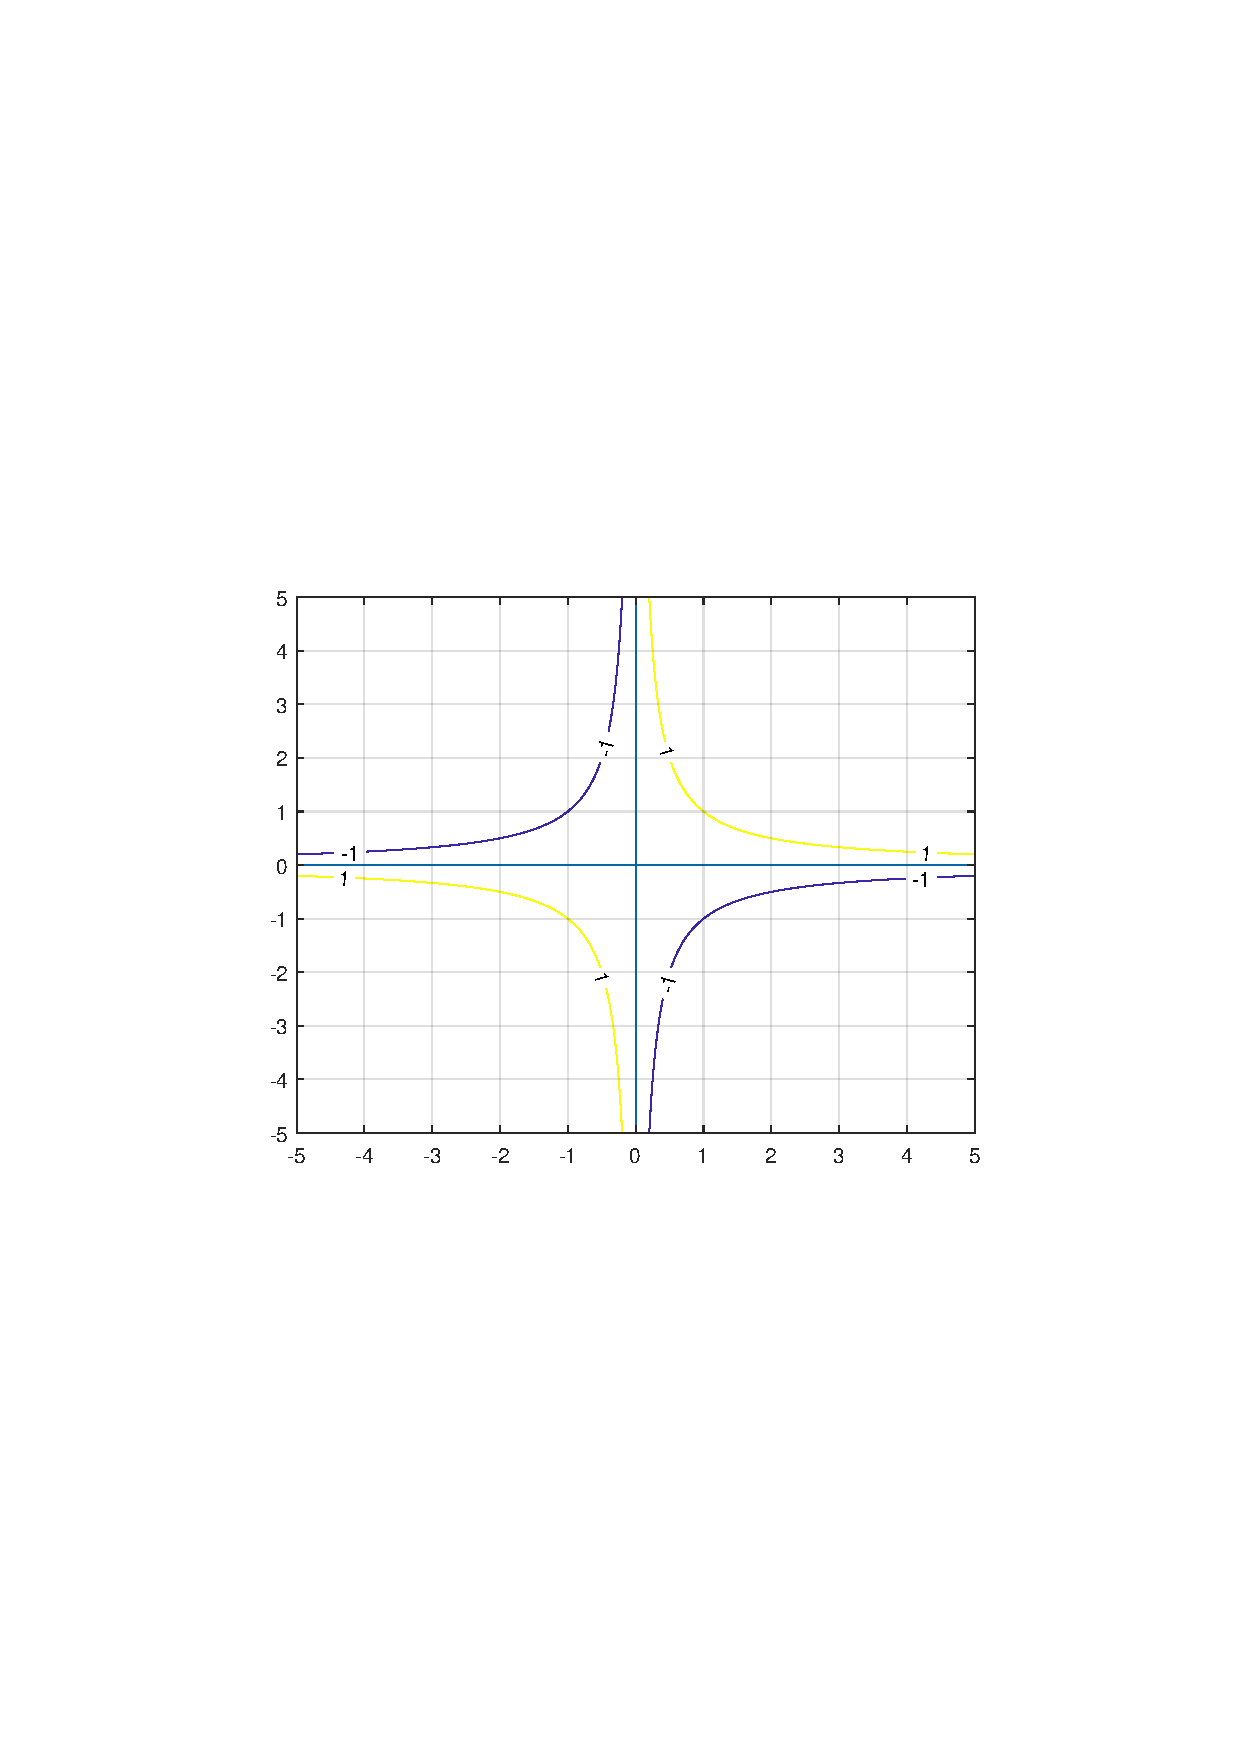
\includegraphics[width=15cm, height=15cm]{../A/analysis/isolines_and_isosurfaces_001_ai.pdf}
%\caption{Isolines of $f_1(x,y) = xy$.}
%\label{f_1}
%\end{center}
%\end{figure}
%
%\begin{figure}[ht]
%\begin{center}
%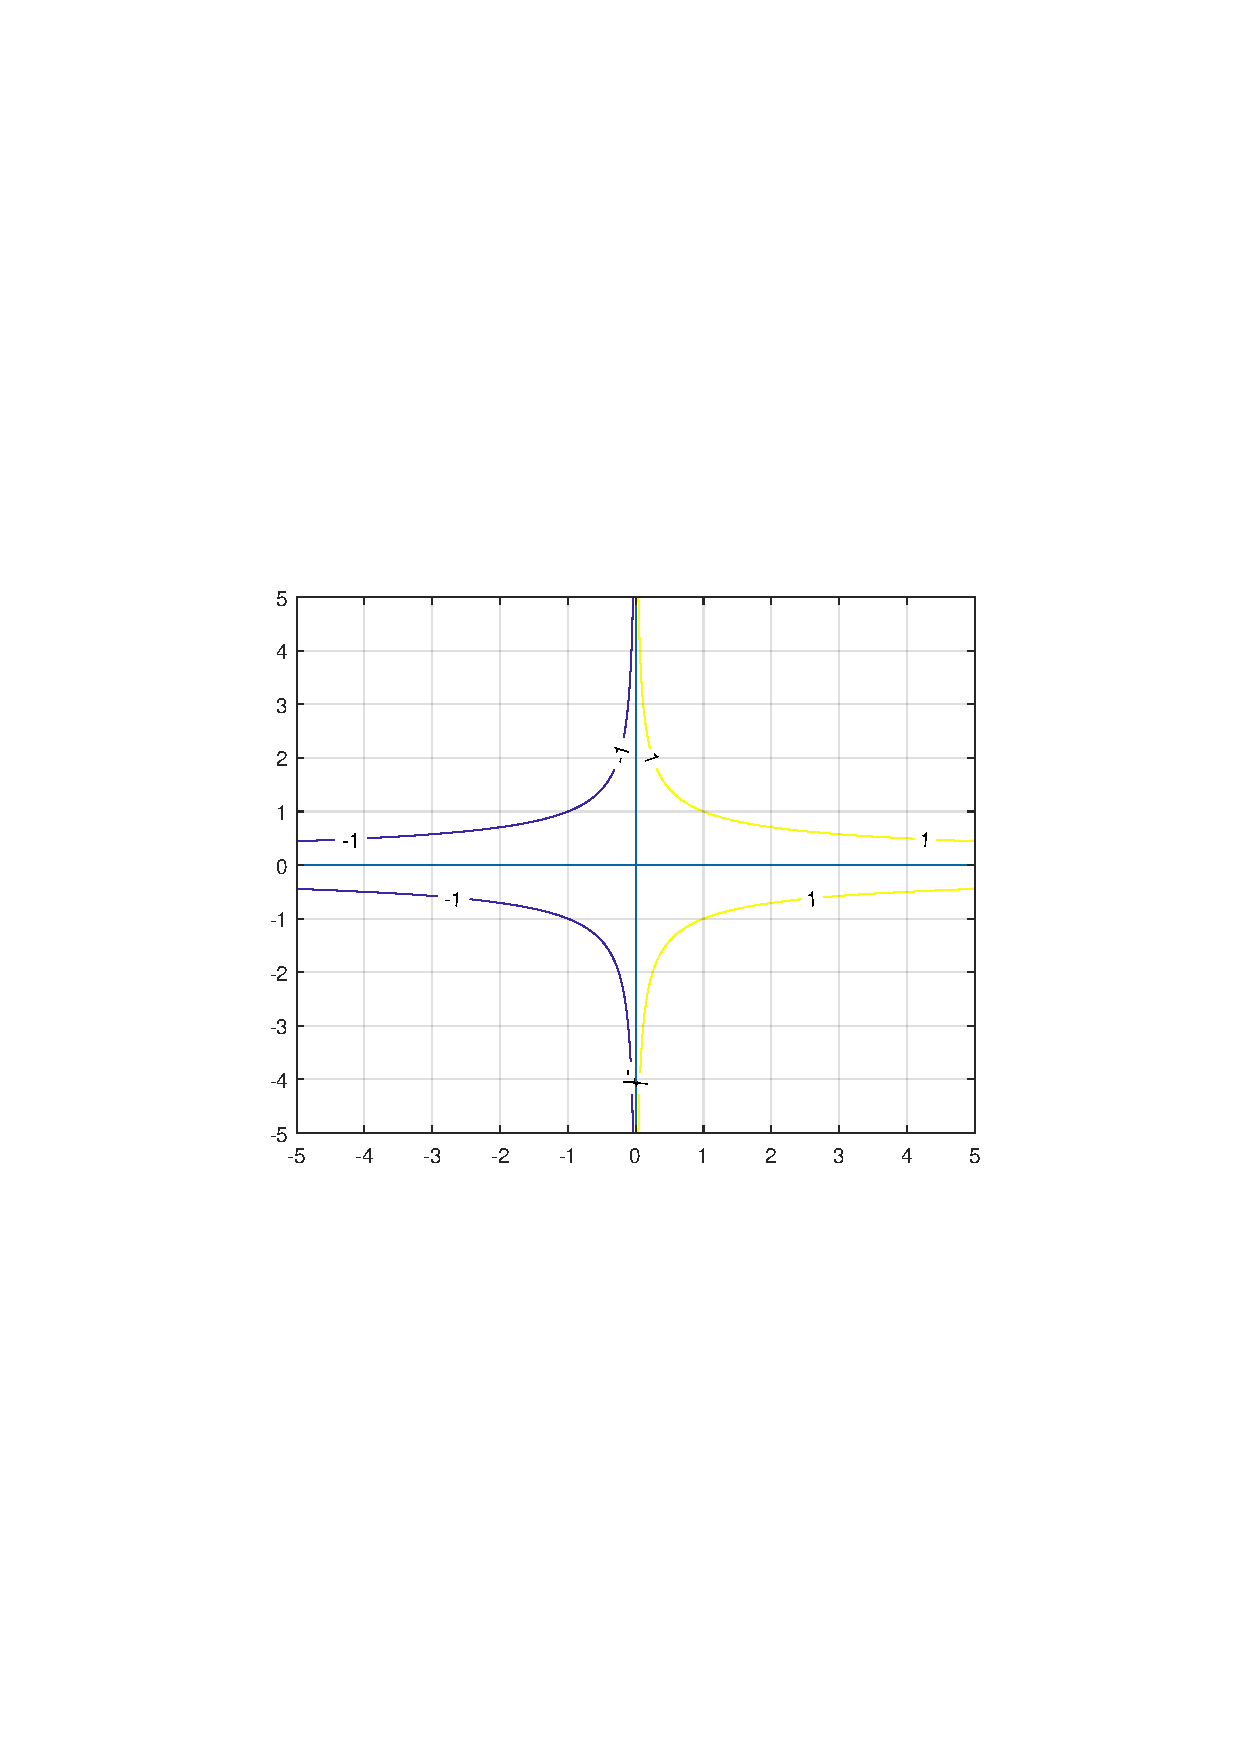
\includegraphics[width=15cm, height=15cm]{../A/analysis/isolines_and_isosurfaces_001_aii.pdf}
%\caption{Isolines of $f_2(x,y) = x^2y$.}
%\label{f_2}
%\end{center}
%\end{figure}
%
%\begin{figure}[ht]
%\begin{center}
%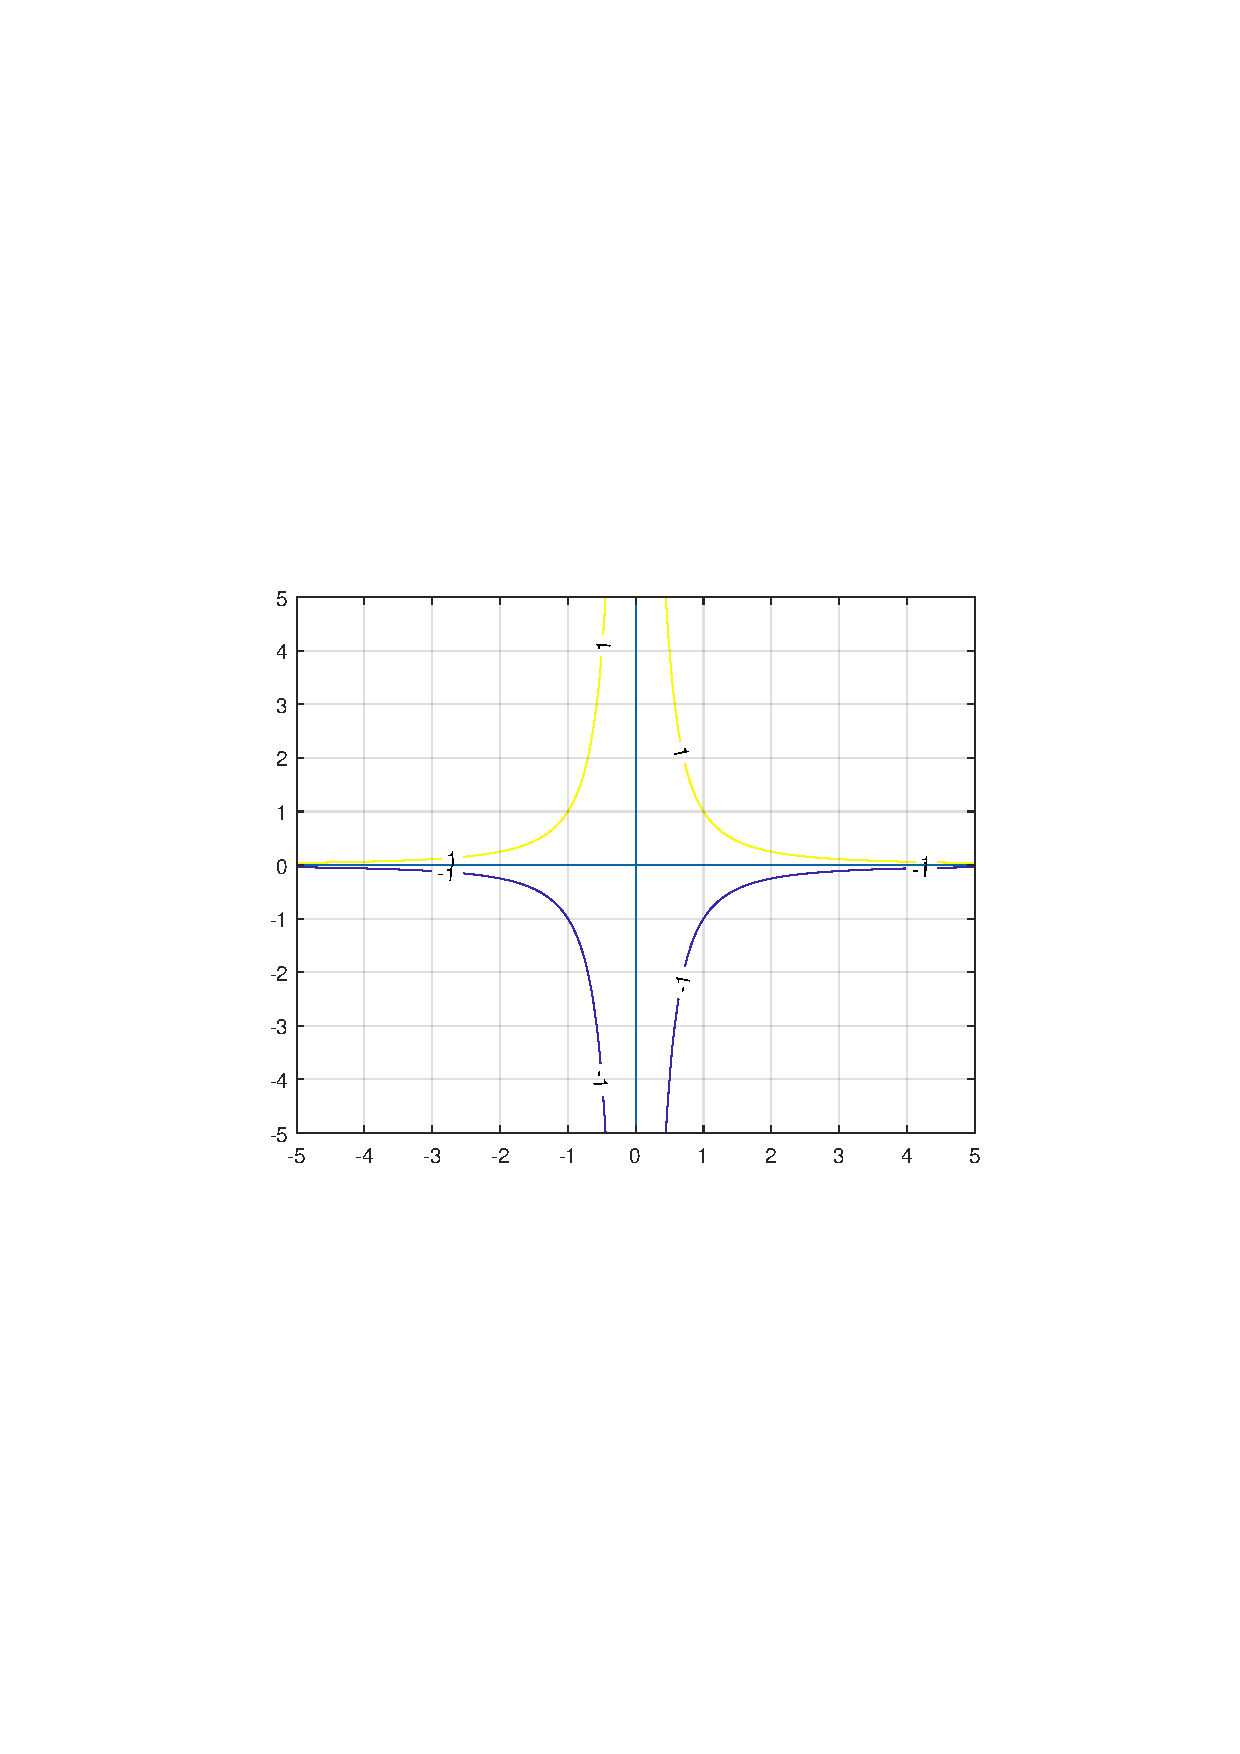
\includegraphics[width=15cm, height=15cm]{../A/analysis/isolines_and_isosurfaces_001_aiii.pdf}
%\caption{Isolines of $f_3(x,y) = xy^2$.}
%\label{f_3}
%\end{center}
%\end{figure}
%
%\begin{figure}[ht]
%\begin{center}
%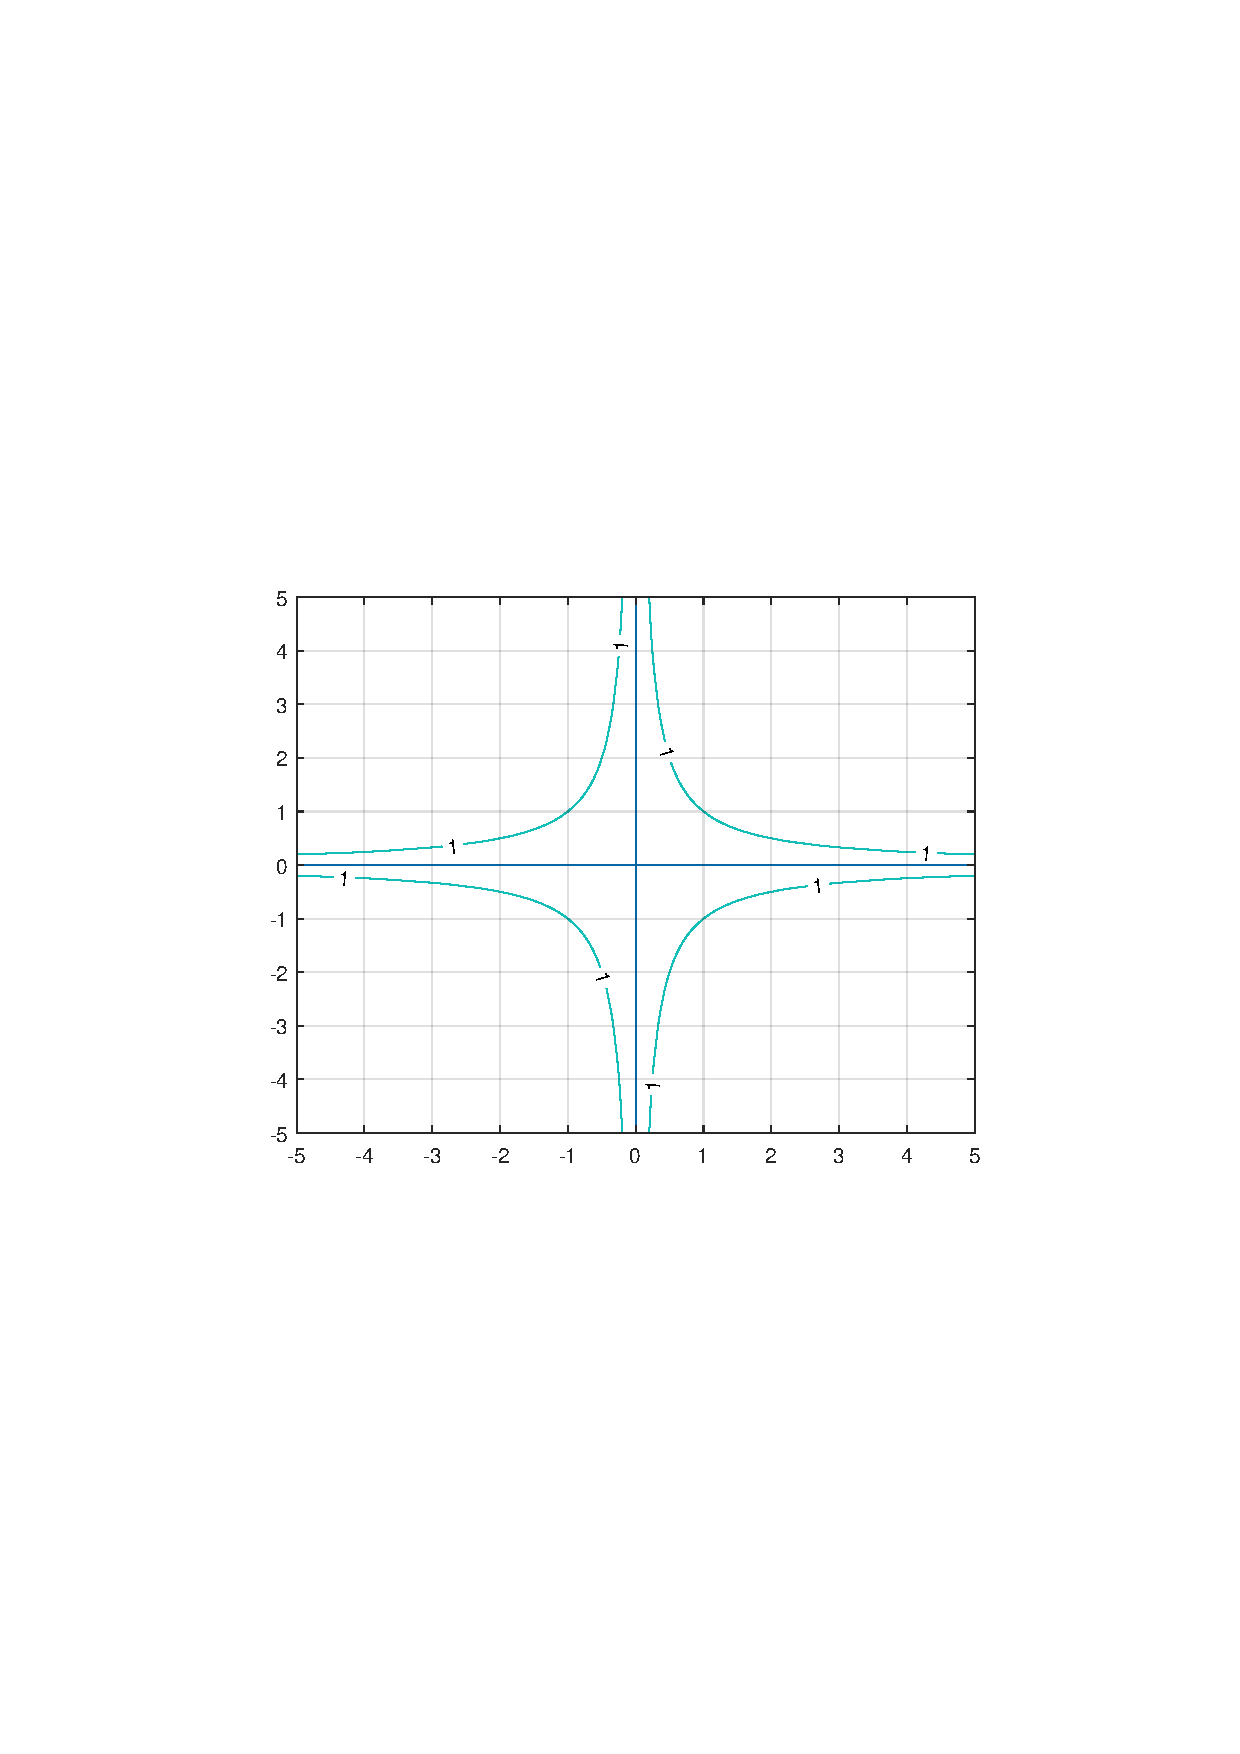
\includegraphics[width=15cm, height=15cm]{../A/analysis/isolines_and_isosurfaces_001_aiv.pdf}
%\caption{Isolines of $f_4(x,y) = x^2y^2$.}
%\label{f_4}
%\end{center}
%\end{figure}


\textbf{b)}
\begin{iii}
\item The function $f_5$ is a paraboloid. The intersection with the plane $z = 0$ is a circle with the radius 1 (see figure \ref{z=0}).\\
The intersection with the plane $z = 1$ is a circle with the radius $\sqrt{2}$ (see figure \ref{z=1}). 
The intersection with the plane $z = -1$ is the point at $(0,0)$ (see figure \ref{z=-1}). 
\item The intersection of the function $f_5$ and the plane $z =2x+2y$ is an ellipse (see figure \ref{z=2x+2y}).
\end{iii}
%\begin{figure}[ht]
%\begin{center}
%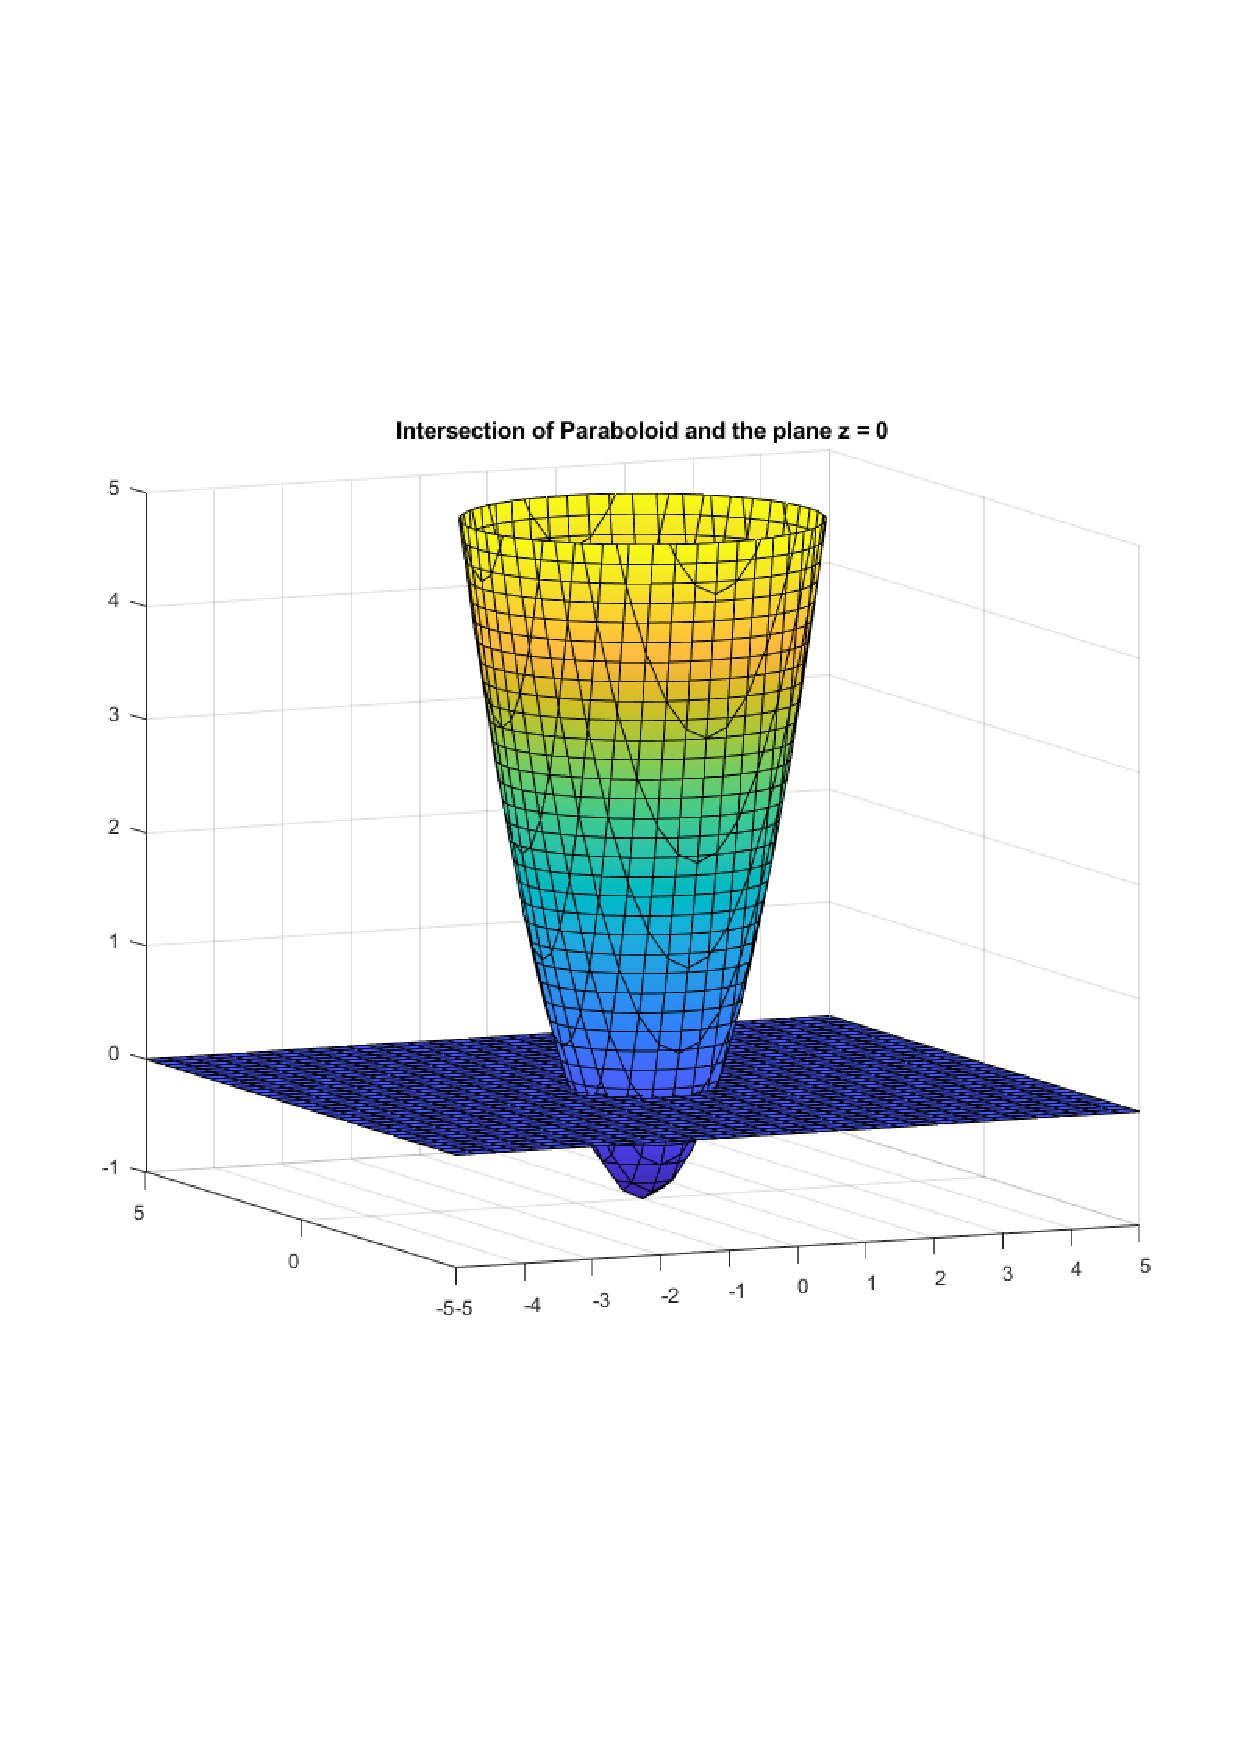
\includegraphics[width=15cm, height=15cm]{../A/analysis/isolines_and_isosurfaces_001_bi1.pdf}
%\caption{Intersection of the paraboloid and the plane $z=0$.}
%\label{z=0}
%\end{center}
%\end{figure}
%
%\begin{figure}[ht]
%\begin{center}
%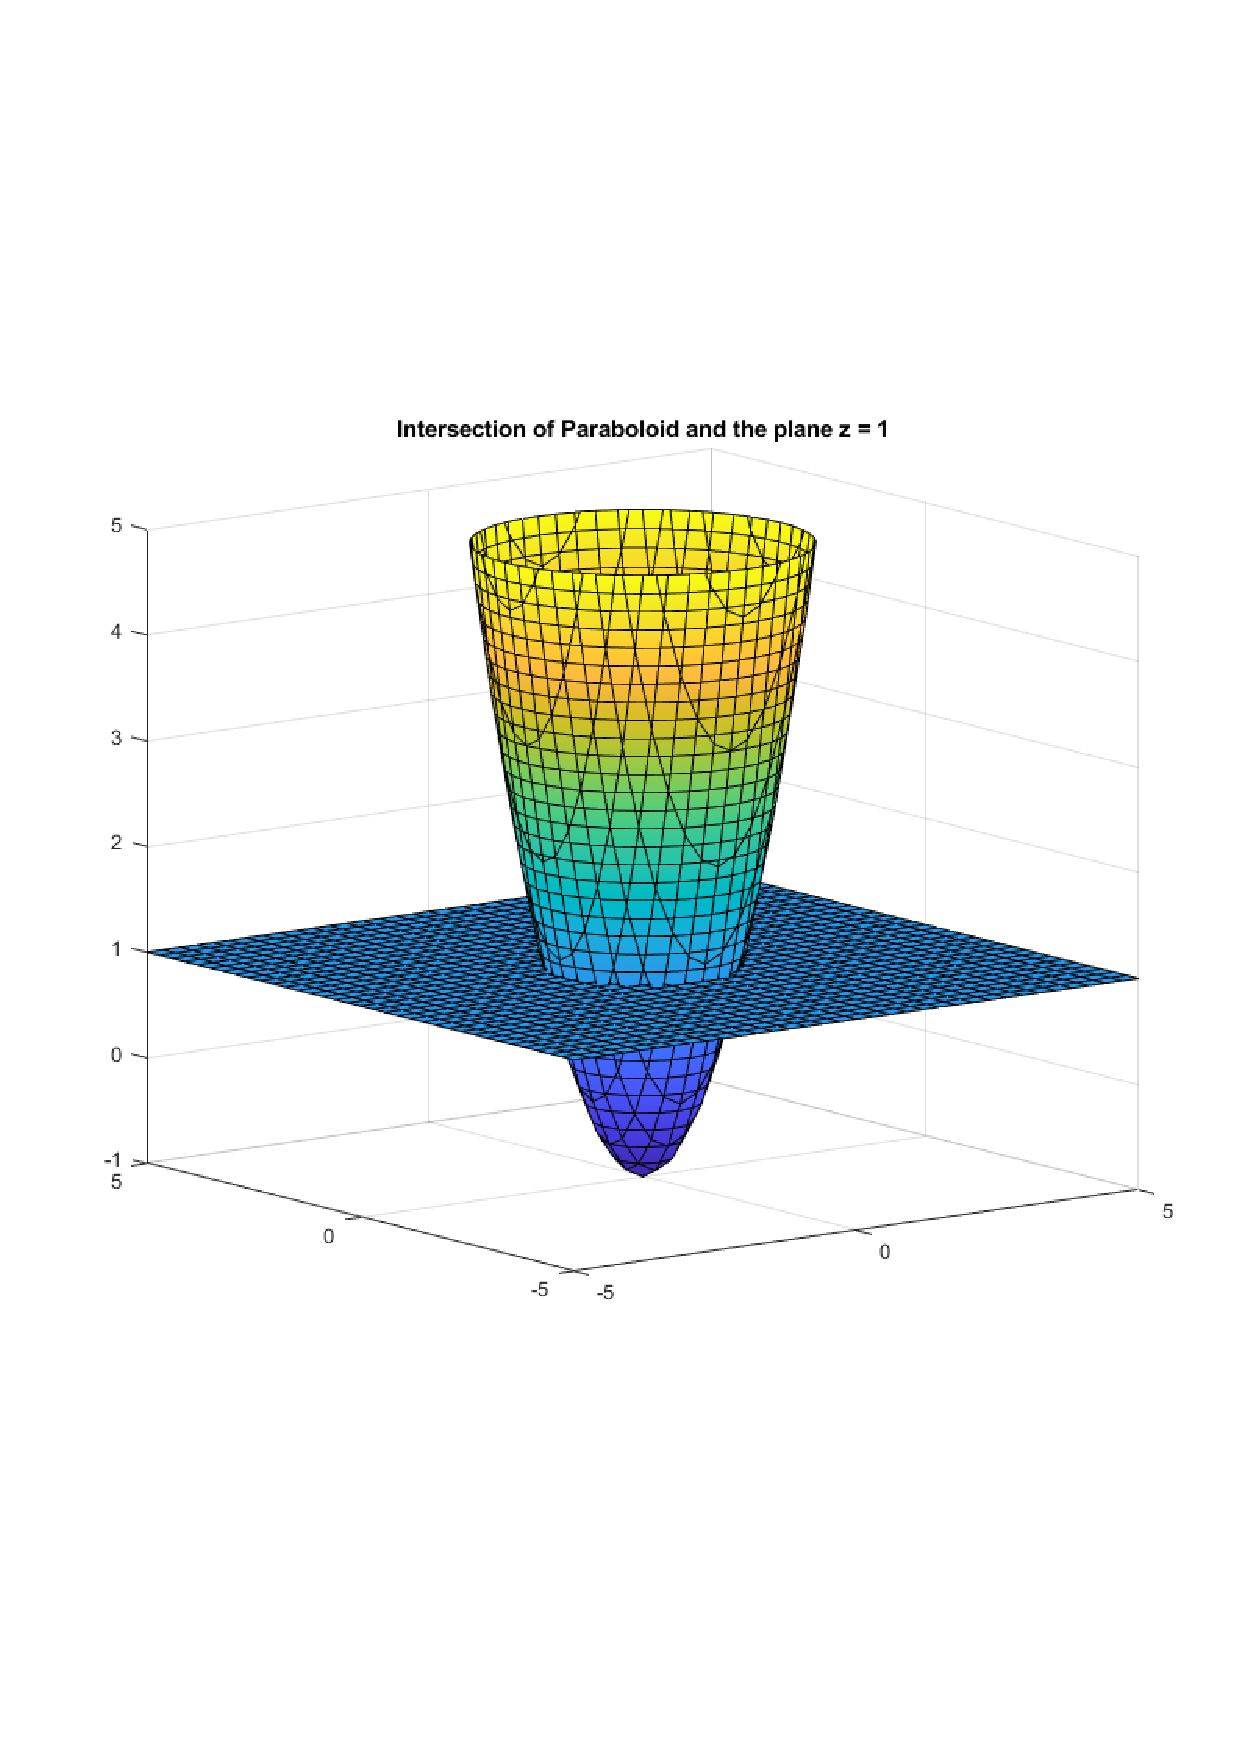
\includegraphics[width=15cm, height=15cm]{../A/analysis/isolines_and_isosurfaces_001_bi2.pdf}
%\caption{Intersection of the paraboloid and the plane $z=1$.}
%\label{z=1}
%\end{center}
%\end{figure}
%
%\begin{figure}[ht]
%\begin{center}
%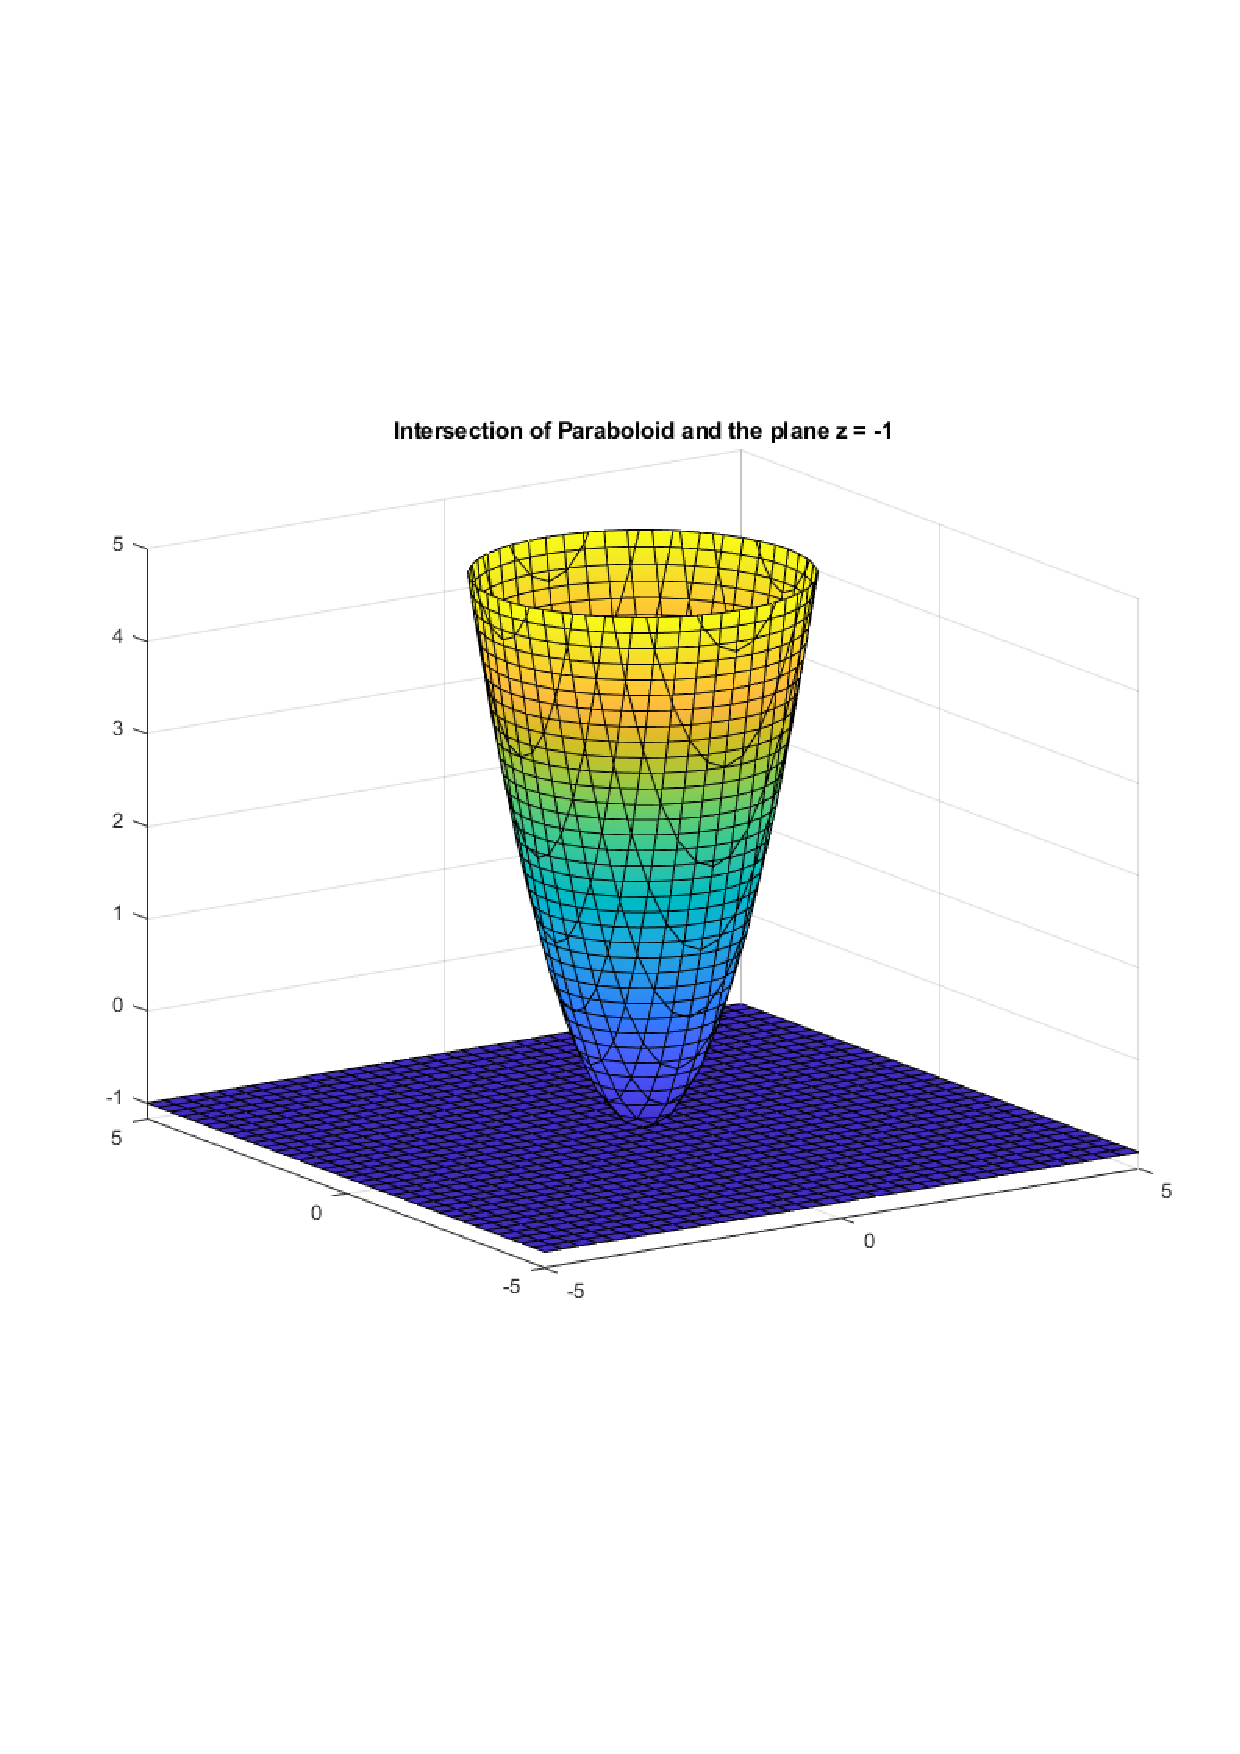
\includegraphics[width=15cm, height=15cm]{../A/analysis/isolines_and_isosurfaces_001_bi3.pdf}
%\caption{Intersection of the paraboloid and the plane $z=-1$.}
%\label{z=-1}
%\end{center}
%\end{figure}
%
%\begin{figure}[ht]
%\begin{center}
%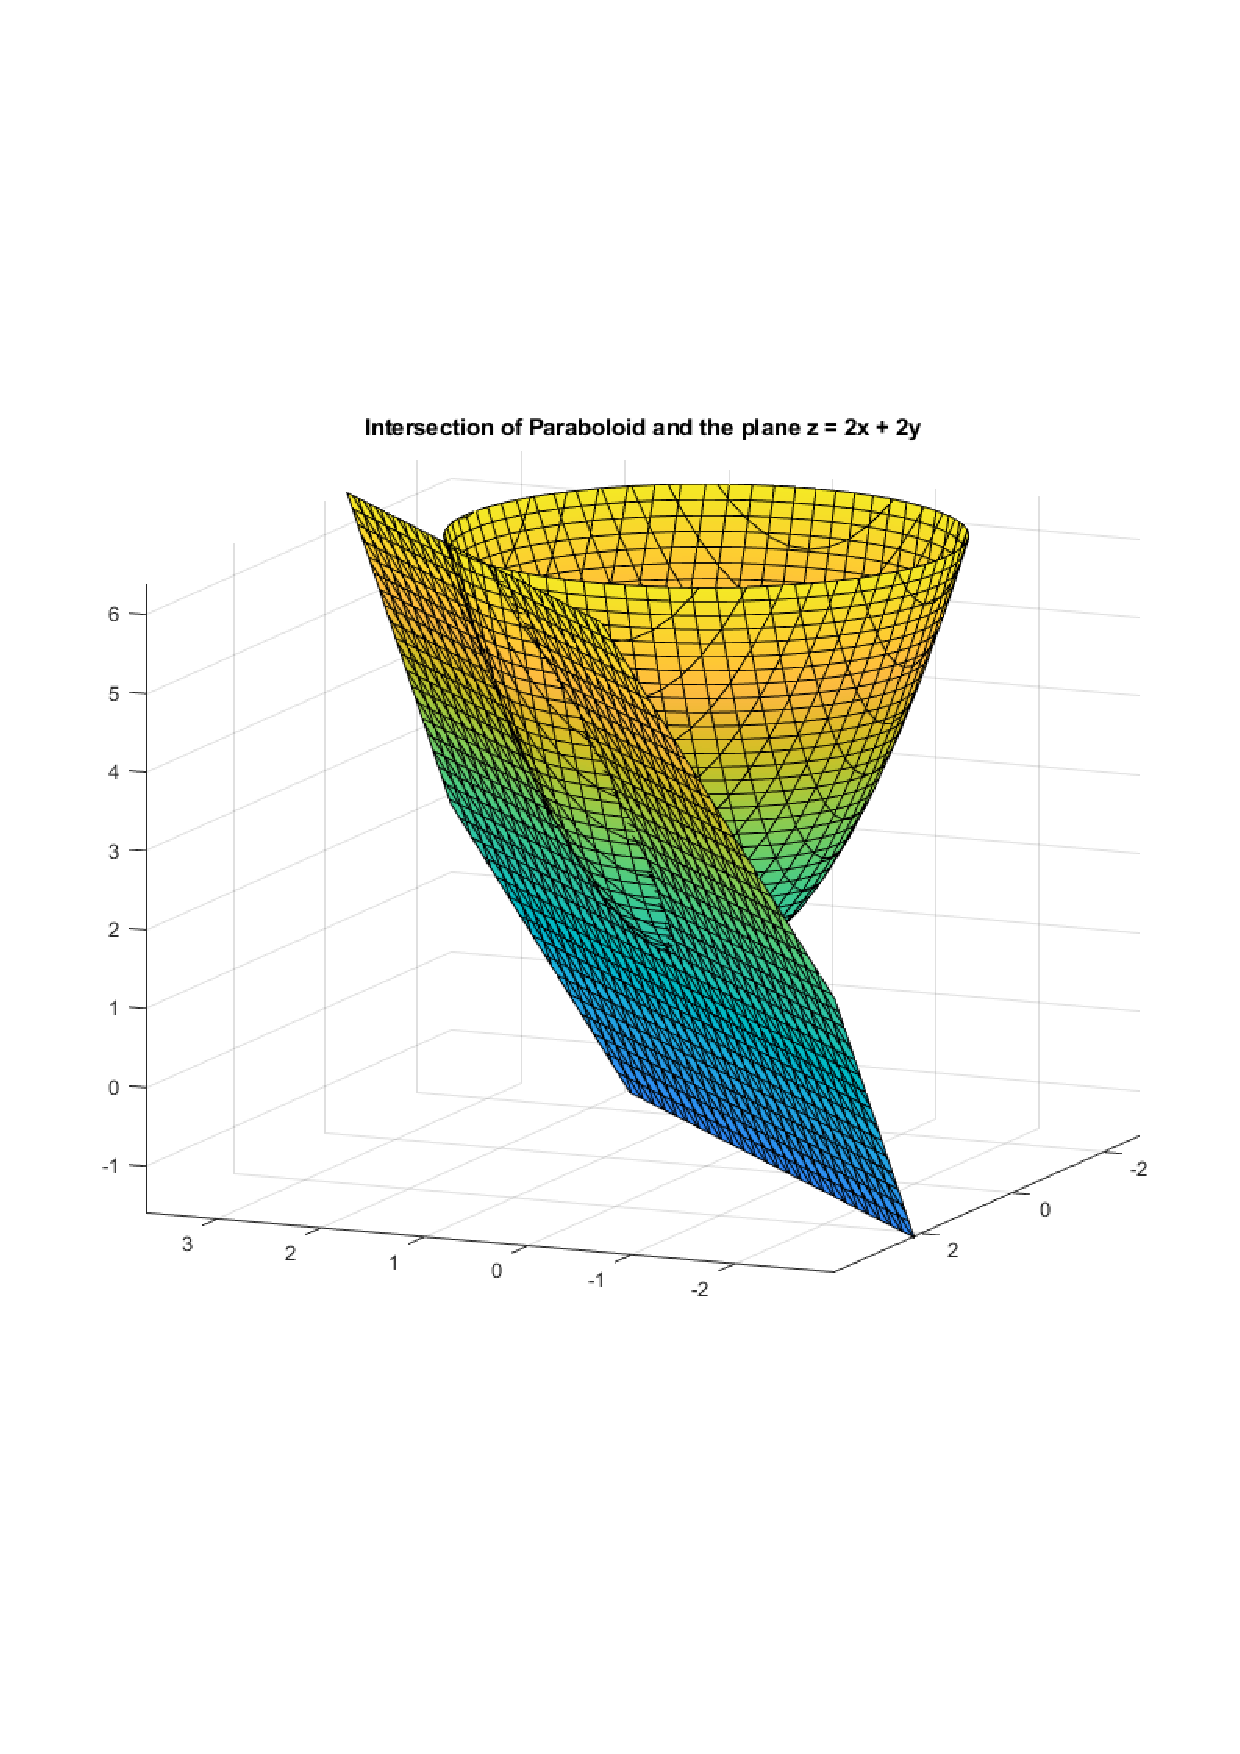
\includegraphics[width=15cm, height=15cm]{../A/analysis/isolines_and_isosurfaces_001_bii.pdf}
%\caption{Intersection of the paraboloid and the plane $z=2x+2y$.}
%\label{z=2x+2y}
%\end{center}
%\end{figure}


}


\ifthenelse{\boolean{mitLoes}}{\ruleBig \cleardoublepage}{}



% \ifthenelse{\boolean{mitLoes}}{\cleardoublepage}{}
\ifthenelse{\boolean{mitErg}}{
\ruleBig
\Ergebnisse}{}


\end{twocolumn}
\end{document}
